\chapter{Introduction}
\section{Lipid bilayer}
In biological system, cell membranes define the boundary of living organism
and surrounding environment. They regulate what can come and leave living
cells. Building blocks of cell membranes are lipid bilayers.
Lipid bilayers are self-assembled system of lipids, which are 
amphiphilic molecules that consist of a hydrophilic headgroup
and hydrophobic chains (Fig.~\ref{fig:lipid}).

\begin{figure}
  \centering
  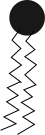
\includegraphics[width=0.2\textwidth]{figures/lipid}
  \caption{Schematic representation of a lipid molecule}
  \label{fig:lipid}
\end{figure}

In water, lipids self-assemble into lipid bilayes to shield their hydrophobic 
cores, and 
display a wide variety of thermodynamic phases
as a function of temperature and hydration. Figure~\ref{fig:phase_diagram}
shows a phase diagram of dimyristoylphosphatidylcholines (DMPC).
PC lipids constitute a substantial fraction of cell membranes
and have been studied for many decades.
At full hydration, a lamellar phase coexists with excess water.
In the high temperature, fluid $L_\alpha$ phase, the hydrocarbon chains 
are conformationally disordered, and intra-membrane molecular correlations 
are liquid-like \cite{ref:Fahey78} (Fig.~\ref{fig:various_phases}).
Disordering of fluid phase membranes allows proteins to 
interact with cell membranes in various ways, rendering biological systems
highly complex. 
This phase is usually considered biologically relevant, making it
the most widely studied phase for understanding various biological processes.

\begin{figure}[htbp]
  \centering
  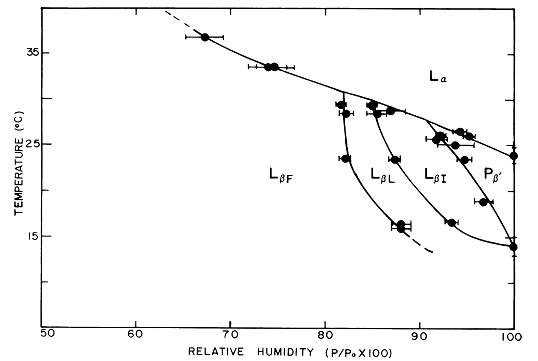
\includegraphics[width=0.9\textwidth]{figures/smith_phase_diagram}
  \caption{Experimental phase diagram of DMPC from Ref.~\cite{ref:Smith88}.
  \LbetaI, \LbetaL, and \LbetaF\ belong to the gel $L_{\beta'}$ phase. $P_{\beta'}$ is 
  the ripple phase and $L_\alpha$ is the fluid phase.}
  \label{fig:phase_diagram}
\end{figure}

\begin{figure}[htbp]
  \centering
  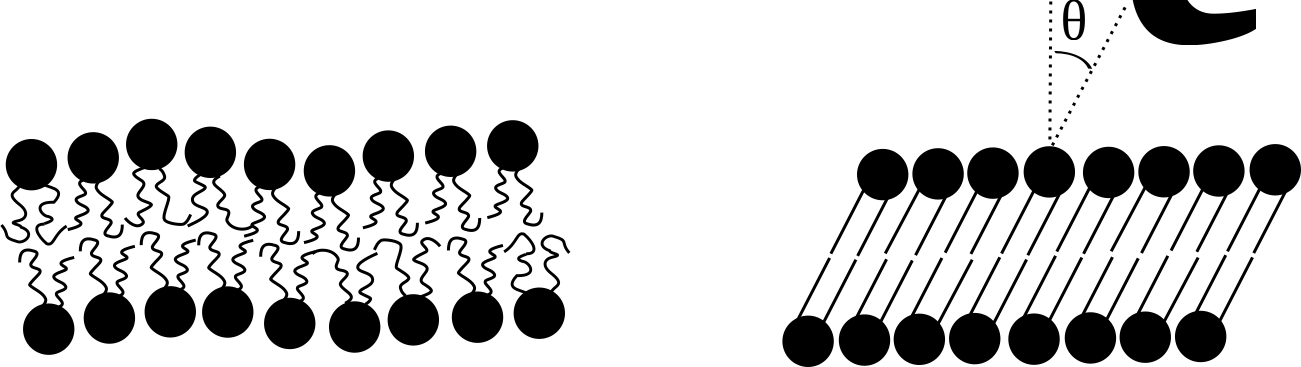
\includegraphics[width=0.9\textwidth]{figures/various_phases}
  \caption[]{Schematics of the structure of fluid $L_\alpha$ phase (left) and 
  gel $L_{\beta'}$ phase (right). Black solid circles are lipid headgroups 
  and solid lines are lipid chains. $\theta_t$ is the chain tilt angle.}
  \label{fig:various_phases}
\end{figure}

In the low temperature, gel $L_{\beta'}$
phase, hydrocarbon chains are stiff and titled with respect to the membrane
normal \cite{ref:Tardieu73}, and are organized in a either hexagonal 
or orthorhombic lattice. 
The $L_{\beta'}$ is further categorized into three phases according to the 
chain tilt direction \cite{ref:Smith88,ref:Tristram93,Tristram-Nagle02}. 
In the $L_{\beta\text{I}}$ phase, chains are titled toward the 
nearest neighbor as shown in Fig.~\ref{fig:gel_phase_packing}, and
in the \LbetaF\ phase, chains are titled toward the next nearest neighbor.
In the \LbetaL\ phase, chains are tilted toward an intermediate direction.

\begin{figure}[htbp]
  \centering
  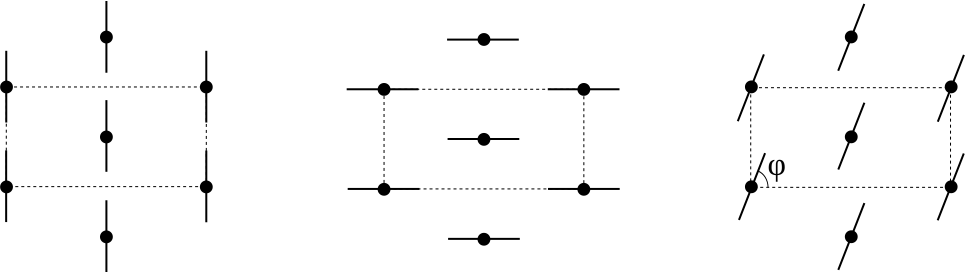
\includegraphics[width=0.9\textwidth]{figures/gel_phase_packing}
  \caption{Chain tilt direction in \LbetaI\ (left), \LbetaF\ (middle), and
  \LbetaL\ (right) phases. Black dots are orthorhombic lattice points.
  Unit cells are shown in dashed lines.
  Chains are drawn as solid lines. Chains are tilted toward the
  nearest neighbor in \LbetaI\ phase with $\phi=\pi/2$. 
  In \LbetaF\ phase, they are titled toward the next nearest neighbor
  ($\phi=0$). In \LbetaL\ phase, $\phi$ can be anywhere between 0 and $\pi/2$.}
  \label{fig:gel_phase_packing}
\end{figure}

There are various kinds of lipids. They can be 
categorized in terms of headgroup, chain saturation, and chain length.
The most studied headgroup is a phosphatidylcholine (PC),
consisting of phosphate and choline groups. Another class of headgroup is
anionic, phosphatidylserin (PS). In cells, electrostatic interaction 
greatly influence biological processes and naturally occurring anionic
lipids have been a focus of studies. More recently, membrane curvature
has attracted many physicists. Phosphatidylethanolamine (PE) is a small 
headgroup, and packing of PE lipids leads to spontaneous membrane curvature.
Many proteins have been found to sense/induce membrane curvature, 
making PE lipids especially attractive for those studies.
Lipid hydrocarbon chains can have one or more double bonds. Lipids
with no double bonds in the chains are called saturated lipids.
An example of such lipids is DMPC and DPPC. DPPC at room temperature
forms a $L_{\beta'}$ gel phase.
Lipids with one double bond
are called mono-unsaturated lipids. Examples of such lipids are DOPC.
Unsaturation lead to packing frustration and lower the melting 
temperature. DOPC at room temperature forms a $L_{\alpha}$ fluid phase.
In mammalian cells, unsaturated chains make up a large number.

\begin{figure}
  \centering
  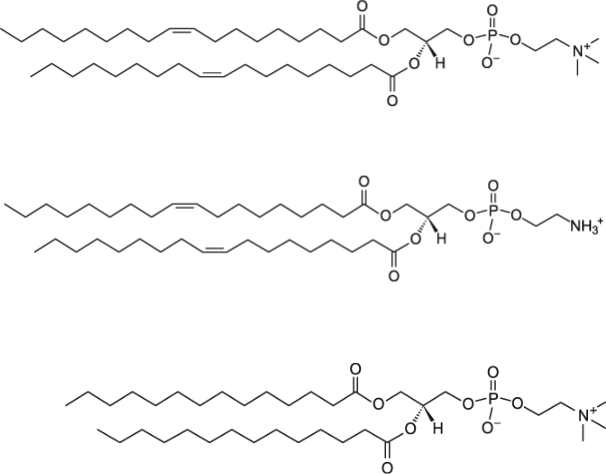
\includegraphics[width=0.7\textwidth]{figures/lipid_structure}
  \caption{Lipid structures of DOPC (top), DOPE (middle),
  and DMPC (bottom). Images are from Avanti Polar Lipids.}
  \label{fig:lipid_structure}
\end{figure}

\section{Tat peptide}
A protein important for infection is produced by the HIV Tat regulatory gene;
after synthesis on the HIV RNA, Tat protein enters the nucleus where it is a
transcriptional transactivator for the long terminal repeat (LTR)
promoter which acts by binding to the Tar RNA element \cite{Vaishnav91}
(Fig.~\ref{fig:HIV_lifecycle}).
A more recently discovered role is that Tat participates in RNA
initiation by stimulating the transcription complex \cite{Raha05}.
Both of these roles activate the HIV virus and increase viral loads.
One focus of current AIDS research is to eradicate reservoirs of 
infected memory T-cells that contain HIV in a latent state;
Tat is capable of awakening latent provirus \cite{Macias09}.
The biomedical significance is that understanding this mechanism of 
Tat transport could lead to treatments to either prevent Tat from
reaching the nuclear genome, or to use Tat to awaken dormant virus
in an effort to eradicate it by standard treatments that only
work with active virus \cite{Macias09}. Of the 86 amino acids in Tat,
the highly basic (Y$_{47}$GRKKRRQRRR$_{57}$) sequence called Tat peptide 
is essential to transport
Tat through the nuclear membrane \cite{Ruben89,Hauber87} as mutations within
this region yield a nonfunctional Tat protein that does not enter the cell 
nucleus. The efficiency of the Tat peptide for translocation through
membranes has made it a model for peptide-aided protein and drug delivery
\cite{Futaki01}. The mechanism of Tat-peptide translocation of proteins, 
DNA, RNA, and drugs through the membrane is of considerable interest
since it it known that desolvating and moving charged groups across membranes
can be energetically prohibitive \cite{Grabe04}. 
It has been suggested by MD simulations that Tat peptide first binds rather
more deeply in the membrane, below the phosphates, than
would be anticipated for such a highly charged peptide. From that position,
Tat may electrostatically attract the phosphates in the distal monolayer
leading to the formation of a transient water-filled pore through which
proteins and drugs diffuse \cite{Herce07}. 
We studied the transverse location of Tat within membranes by X-ray scattering
combined with MD simulations. This study is described in chapter 2.

\begin{figure}
  \centering
  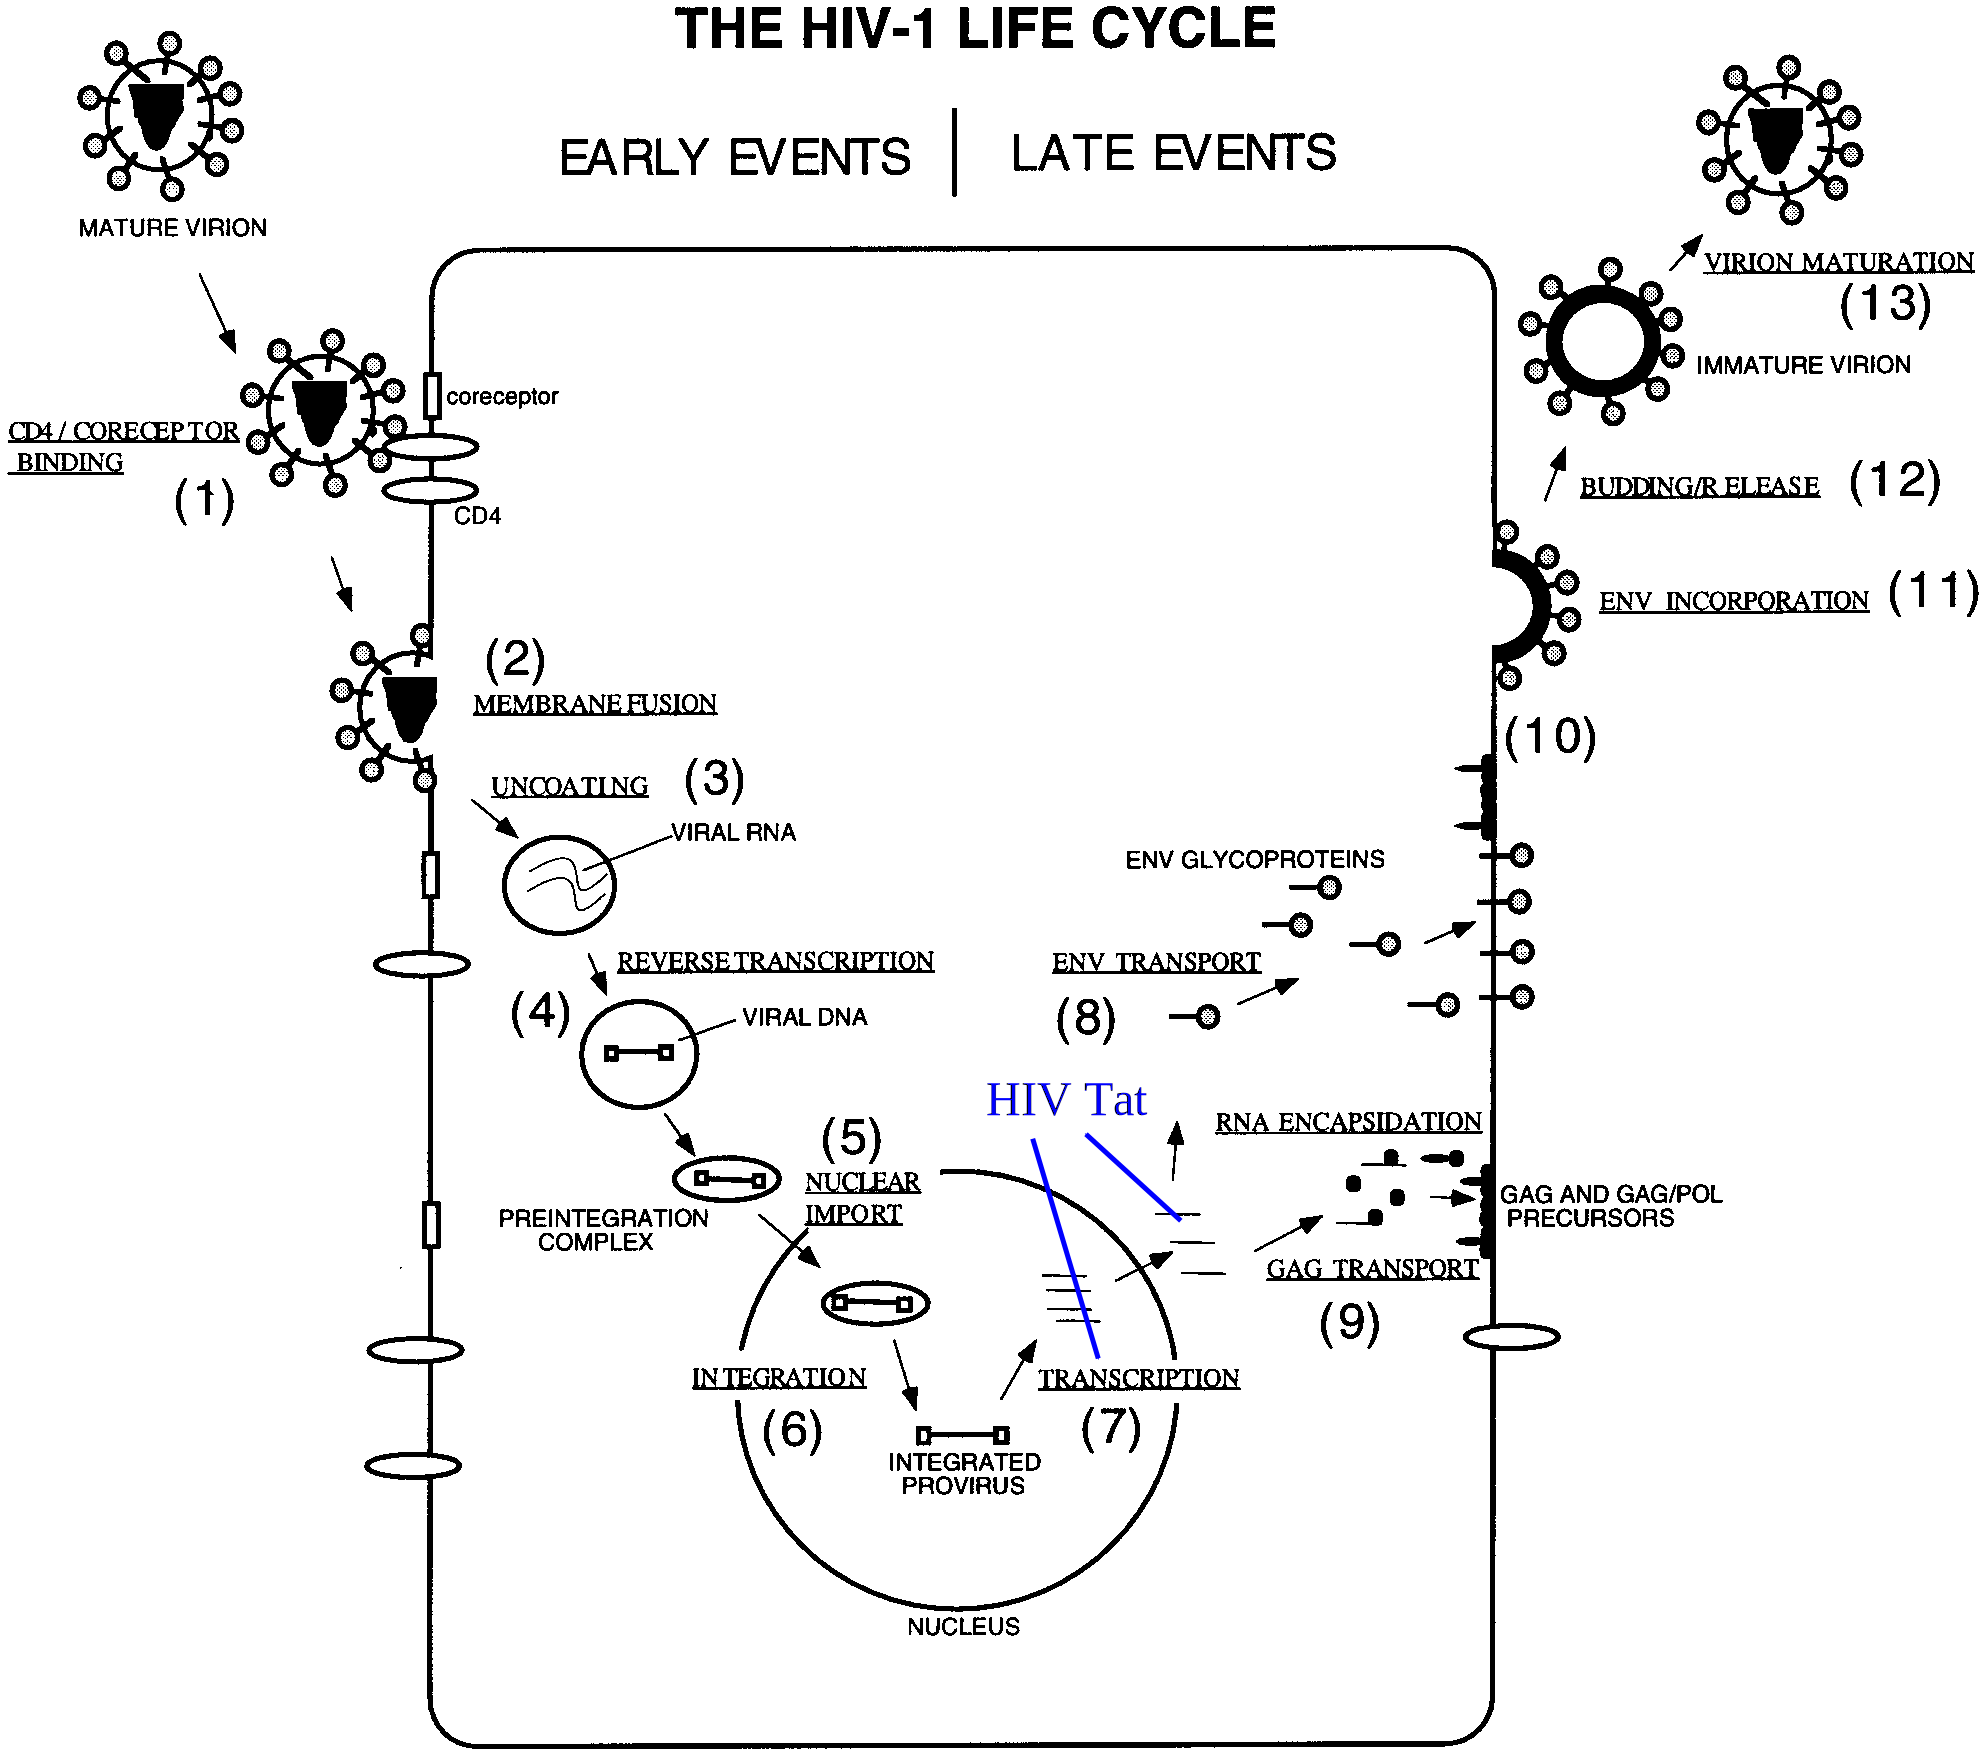
\includegraphics[width=\textwidth]{figures/HIV_lifecycle}
  \caption{HIV-1 life cycle, adapted from Ref.~\cite{Freed98}
  (additions in blue).}
  \label{fig:HIV_lifecycle}
\end{figure}

\section{$P_{\beta'}$ ripple phase}
Between the fluid and gel phases appears a height modulated phase where
bilayers are no longer flat (Fig.~\ref{fig:ripple_cartoon}). 
The low angle diffraction pattern of this phase conforms to the symmetry
of a two dimensional monoclinic lattice. This phase was termed $P_\beta'$ 
and is commonly
called the ripple phase. The $P_{\beta'}$--$L_{\beta'}$ transition is often
called the pre-transition.
The topography of the membrane ripples has been directly
visualized by freeze fracture electron microscopy experiments 
\cite{ref:Luna77,ref:Copeland80,ref:Ruppel83,ref:Zasadzinski87,ref:Zasadzinski88}.
The wavelength of the modulation is about 140 \AA\ for 
dimyristoylphosphatidylcholine (DMPC),
which has 14 carbons in the hydrocarbon chains \cite{ref:Wack89}.
There has been evidence that molecular conformation in the ripple phase is not 
unique. NMR signals in the ripple phase \cite{ref:Wittebort81} were consistent
with a superposition of signals observed in the fluid and gel phases.
Lateral diffusion measurements found two distinct populations,
with diffusion coefficients characteristic of fluid and gel phases
\cite{ref:Schneider83}. 
We studied electron density distribution and chain packing 
of the asymmetric DMPC ripple phase using low and wide angle X-ray scattering.
The ripple phase is discussed in chapter 3. 

\begin{figure}[htbp]
  \centering
  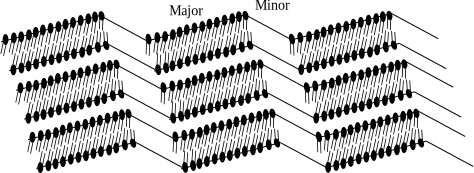
\includegraphics[width=0.7\textwidth]{figures/ripple_cartoon}
  \caption{Schematic of the $P_{\beta'}$ ripple phase. In this phase, 
  bilayers assume periodic height modulation with a sawtooth shape.
  The longer side of a sawtooth is called major arm and the shorter
  side is called minor arm. It is generally assumed that chains are
  in all trans conformation in the major arm, but the molecular packing
  in the minor arm is not known.}
  \label{fig:ripple_cartoon}
\end{figure}